\documentclass{article}
\RequirePackage[utf8]{vietnam}

\usepackage[fontsize=13pt]{scrextend}
\usepackage[paperheight=29.7cm,paperwidth=21cm,right=2cm,left=3cm,top=2cm,bottom=2.5cm]{geometry}
\usepackage{mathptmx} %Times New Roman
\usepackage{graphics}
\usepackage{float} %Vị trí của hình
\usepackage{tikz} %Vẽ hình
\usetikzlibrary{calc}  
\usepackage{indentfirst} %Thư viện cho những cái ở dưới
\renewcommand{\baselinestretch}{1.2}%Giãn dòng 1.2
\setlength{\parskip}{6pt}%Giãn dòng giữa các đoạn
\setlength{\parindent}{1cm}%Khoảng cách thụt đầu dòng mỗi đoạn
\usepackage{titlesec}%Thư viện set up kiểu chữ
\stepcounter{secnumdepth}%Đánh số thứ tự cho các section
\titlespacing*{\section}{0pt}{0pt}{30pt} %Heading 1
\titleformat*{\section}{\fontsize{16pt}{0pt}\selectfont\bfseries\centering}
\titlespacing*{\subsection}{0pt}{10pt}{0pt} %Heading 2
\titleformat*{\subsection}{\fontsize{14pt}{0pt}\selectfont\bfseries}
\titlespacing*{\subsubsection}{0pt}{10pt}{30pt} %Heading 3
\titleformat*{\subsubsection}{\fontsize{13pt}{0pt}\selectfont\itshape}
\titlespacing*{\paragraph}{10pt}{0pt}{0pt} %Heading 4
\titleformat*{\paragraph}{\fontsize{13pt}{0pt}\selectfont\itshape}
\titlespacing*{\subsubsection}{0pt}{*0}{*0.5}%Khoảng cách giữa các heading của subsubsection
\definecolor{customblue}{rgb}{0.0, 0.5, 1.0}

\begin{document}

\begin{titlepage}
    \begin{tikzpicture}[overlay,remember picture]
        \draw [line width=5pt, draw=customblue]
        ($ (current page.north west) + (3cm,-2cm) $)
        rectangle
        ($ (current page.south east) + (-2cm,2.5cm) $);
        \draw [line width=0.5pt]
        ($ (current page.north west) + (3.1cm,-2.1cm) $)
        rectangle
        ($ (current page.south east) + (-2.1cm,2.6cm) $);
    \end{tikzpicture}

    \begin{center}
        \vspace{-0.5cm}
        TRƯỜNG ĐẠI HỌC BÁCH KHOA \\
        ĐẠI HỌC QUỐC GIA THÀNH PHỐ HỒ CHÍ MINH \\
        KHOA CƠ KHÍ \\


    \begin{figure}[H]
        \centering
        
\includegraphics[width=0.3\textwidth]{image/bachkhoa_logo.png}     
    \end{figure}
    \textbf{\fontsize{14pt}{1}\selectfont BÁO CÁO} \\
    \vspace{1cm}
    \textbf{\fontsize{16pt}{1}\selectfont TRANG BỊ ĐIỆN - ĐIỆN TỬ TRONG MÁY CÔNG NGHIỆP} \\
    \vspace{0.5cm}
    \textbf{\fontsize{16pt}{1}\selectfont ĐỀ TÀI: THIẾT KẾ PCB} \\
    \end{center}\
    \vspace{2cm}
    \begin{table}[H]
        \centering
        \begin{tabular}{l l l}
            \textbf{Giáo viên hướng dẫn:} & DƯƠNG VĂN TÚ \vspace{0.5cm} \\ 
            \textbf{Sinh viên thực hiện:} & DƯƠNG QUANG DUY & 2210497\\
                            & VÕ HỮU DƯ & 2210604\\
                            & ĐÀO TRỌNG CHÂN & 2210350\\   
        \end{tabular}
    \end{table}
    \vspace{3.5cm}
    \begin{center}
        \textit{\fontsize{14pt}{1}\selectfont TP. HỒ CHÍ MINH, THÁNG 10/2024}
    \end{center}
\end{titlepage}
\cleardoublepage



\addtocontents{toc}{\protect\thispagestyle{empty}} %Loại bỏ số trang trong mục lục
\tableofcontents %Tạo mục lục tự động
\thispagestyle{empty}
\pagenumbering{Roman} %Bắt đầu đánh số thứ tự la mã
\cleardoublepage

\pagenumbering{arabic} %Bắt đầu đánh số thứ tự số
\section*{CHƯƠNG 1: TÌM HIỂU VỀ PHẦN MỀM ALTIUM DESIGNER}
\stepcounter{section}
\addcontentsline{toc}{section}{\numberline{}CHƯƠNG 1: TÌM HIỂU VỀ PHẦN MỀM ALTIUM DESIGNER}
\subsection{Tìm hiểu về phần mềm Altium Designer}
Altium Designer là một trong những phần mềm chuyên ngành cho phép thiết kế mạch điện tử PCB (Printed Circuit Board). Altium Designer là một phần mềm mạnh với nhiều tính năng. Một số tính năng cơ bản của phần mềm Altium Designer có thể kể đến như sau:
\begin{itemize}
    \item Giao diện thiết kế, quản lý và chỉnh sửa thân thiện, dễ dàng biên dịch, quản lý file, quản lý phiên bản cho các tài liệu thiết kế.
    \item Hỗ trợ mạnh mẽ cho việc thiết kế tự động, đi dây tự động theo thuật toán tối ưu, phân tích lắp ráp linh kiện. Hỗ trợ việc tìm các giải pháp thiết kế hoặc chỉnh sửa mạch, linh kiện, netlist có sẵn từ trước theo các tham số mới.
    \item Mở, xem và in các file thiết kế mạch dễ dàng với đầy đủ các thông tin linh kiện, netlist, dữ liệu bản vẽ, kích thước, số lượng…
    \item Hệ thống các thư viện linh kiện phong phú, chi tiết và hoàn chỉnh bao gồm tất cả các linh kiện nhúng, số, tương tự…
    \item Đặt và sửa đối tượng trên các lớp cơ khí, định nghĩa các luật thiết kế, tùy chỉnh các lớp mạch in, chuyển từ schematic sang PCB, đặt vị trí linh kiện trên PCB.
    \item Mô phỏng mạch PCB 3D, đem lại hình ảnh mạch điện trung thực trong không gian 3 chiều, hỗ trợ MCAD-ECAD, liên kết trực tiếp với mô hình STEP, kiểm tra khoảng cách cách điện, cấu hình cho cả 2D và 3D.
    \item Hỗ trợ thiết kế PCB sang FPGA và ngược lại.
\end{itemize}
\begin{figure}[H]
    \centering
    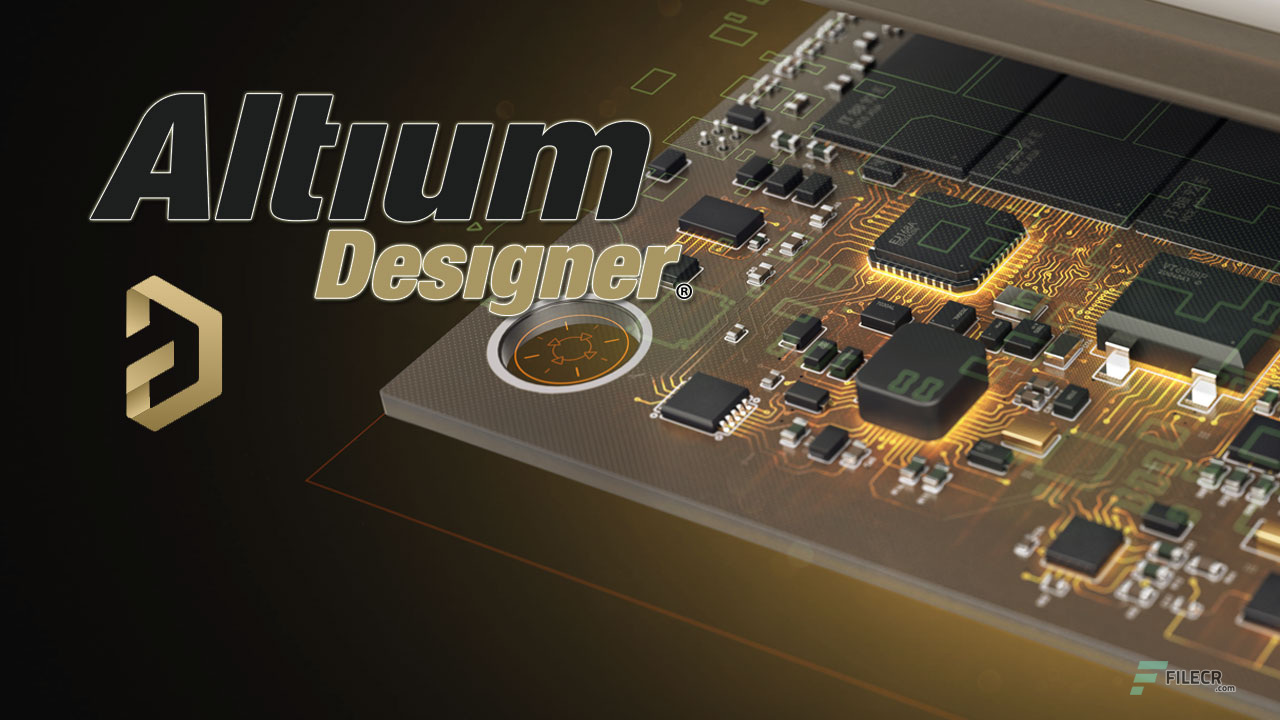
\includegraphics[width=0.6\textwidth]{image/altium.png}
    \caption{Phần mềm Altium Designer}
    \label{fig:altium}
\end{figure}
\cleardoublepage
\subsection{Trình tự thiết kế mạch bằng phần mềm Altium Designer}
\begin{enumerate}
    \item Thiết kế sơ đồ nguyên lí
    \item Lựa chọn các linh kiện phù hợp
    \item Lựa chọn các chân linh kiện để chuyển sang mạch in
    \item Update mạch nguyên lý sang mạch in
    \item Lựa chọn kích thước mạch in, giới hạn mạch in và thiết lập lớp phủ đất
    \item Sắp xếp các vị trí các loại linh kiện như điện trở, tụ điện, IC,…
    \item Đặt luật đi dây, các lỗ via, khoảng cách giữa các linh kiện, lỗ và dây
    \item Đi dây trên mạch và phủ đồng
    \item Kiểm tra toàn mạch
\end{enumerate}
\begin{figure}[H]
    \centering
    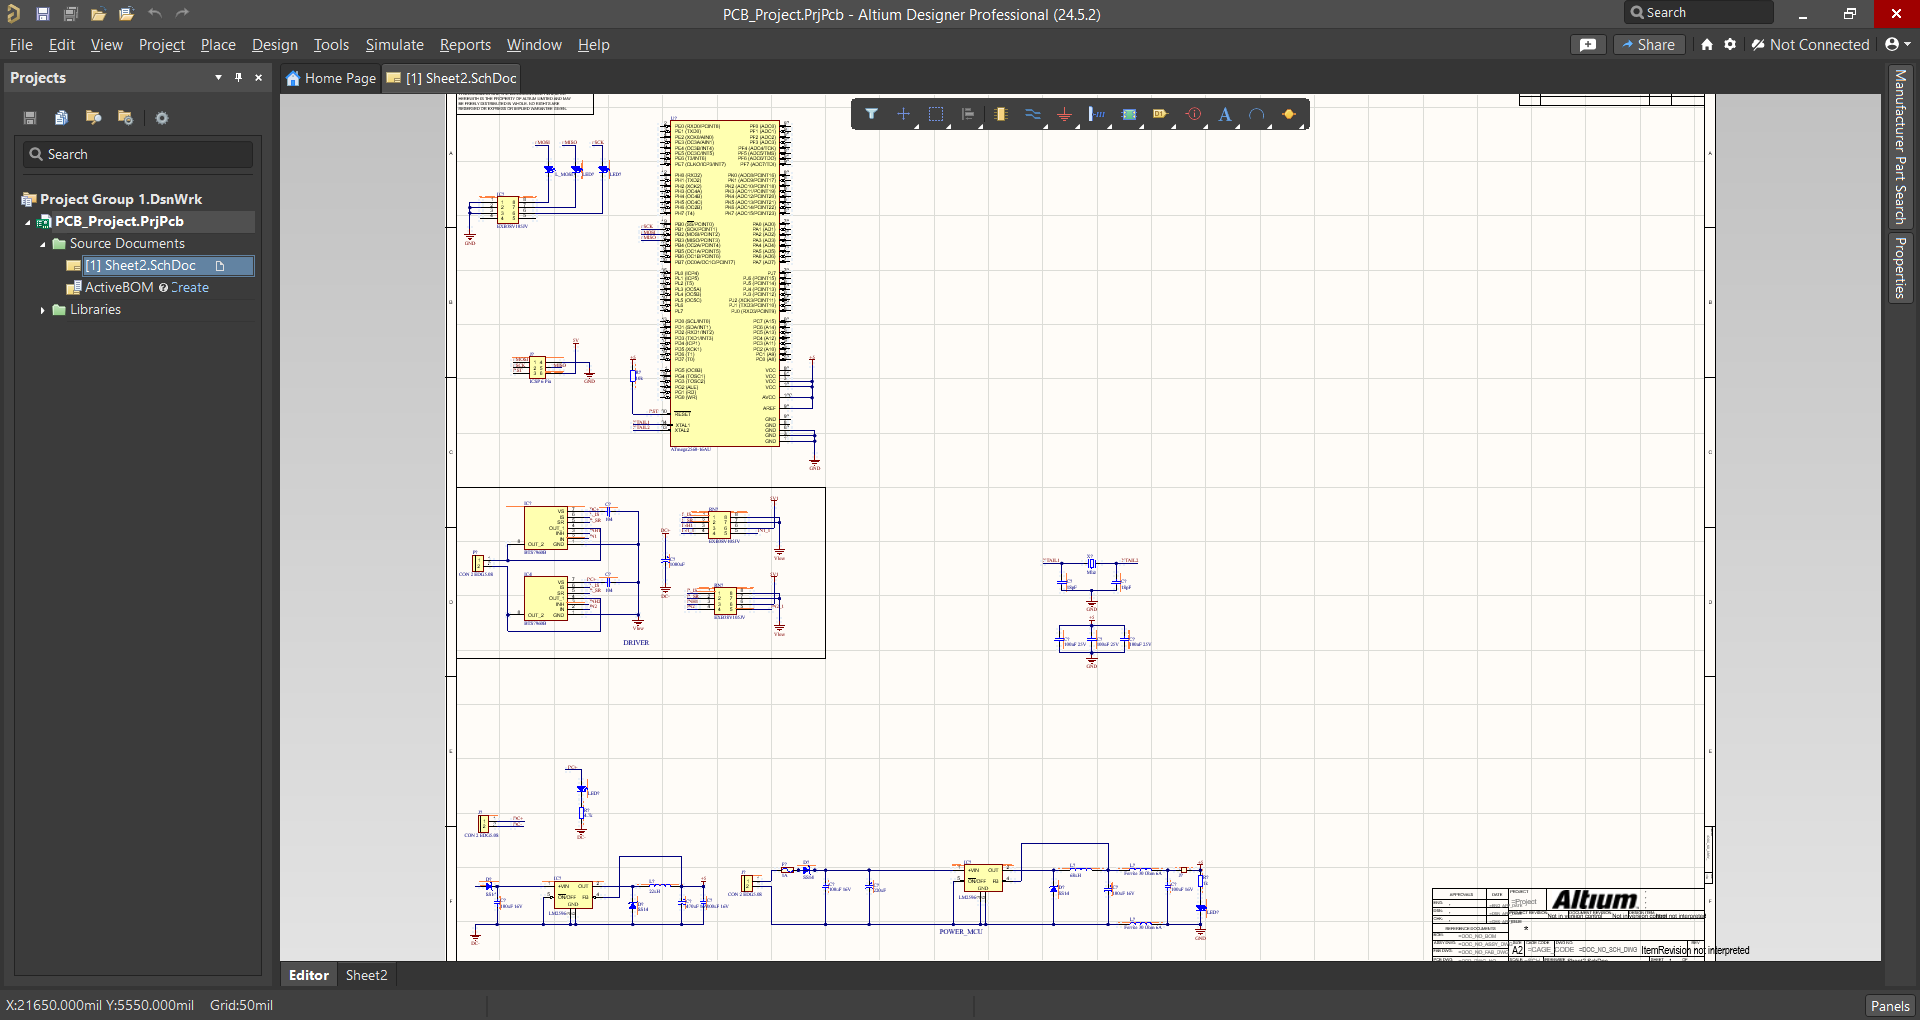
\includegraphics[width=1\textwidth]{image/workspacealtium.png}
    \caption{Giao diện làm việc của phần mềm Altium Designer}
    \label{fig:workspacealtium}
\end{figure}
\cleardoublepage
\subsection{Sơ đồ nguyên lý}
\subsubsection{Sơ lược về sơ đồ nguyên lý}
    Sơ đồ nguyên lý trong mạch điện tử là một biểu đồ biểu diễn các thành phần của
mạch điện và cách chúng được kết nối với nhau. Mục tiêu là để mô tả chức năng của
mạch một cách rõ ràng và dễ hiểu. Các thành phần phổ biến trong sơ đồ nguyên lý của
mạch điện tử bao gồm:
\begin{itemize}
    \item Điện trở (Resistor): Ký hiệu bằng hình chữ nhật hoặc zigzag. Điện trở được sử dụng để giới hạn dòng điện hoặc phân chia điện áp.
    \item Tụ điện (Capacitor): Ký hiệu bằng hai đường thẳng song song. Tụ điện lưu trữ và phóng điện năng.
    \item Cuộn cảm (Inductor): Ký hiệu bằng một loạt các vòng xoắn. Cuộn cảm lưu trữ năng lượng trong từ trường khi dòng điện chạy qua.
    \item Điốt (Diode): Ký hiệu bằng một tam giác và một vạch đứng. Điốt cho phép dòng điện chạy theo một chiều duy nhất.
    \item Transistor:
    \begin{itemize}
        \item NPN: Ký hiệu bằng một mũi tên chỉ ra ngoài từ đường nối giữa base và emitter.
        \item PNP: Ký hiệu bằng một mũi tên chỉ vào trong.
    \end{itemize}
    \item IC (Integrated Circuit): Ký hiệu bằng một hình chữ nhật với nhiều chân ra. IC chứa nhiều linh kiện điện tử tích hợp bên trong.
    \item Nguồn điện (Power Supply): Ký hiệu bằng hai đường thẳng song song, với một đường dài hơn (dương) và một đường ngắn hơn (âm).
\end{itemize}
\subsubsection{Ví dụ về sơ đồ nguyên lý}
\begin{figure}[H]
    \centering
    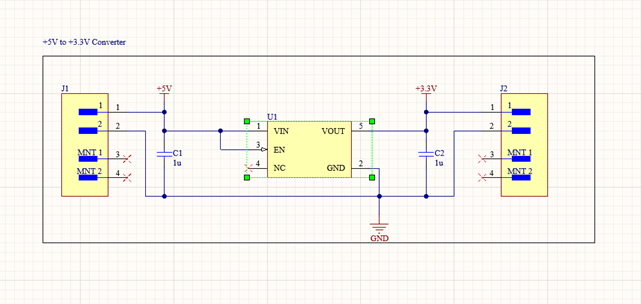
\includegraphics[width=1\textwidth]{image/sch1.png}
    \caption{Sơ đồ nguyên lý mạch chuyển đổi điện áp}
    \label{fig:sodonguyenly}
\end{figure}
\begin{figure}[H]
    \centering
    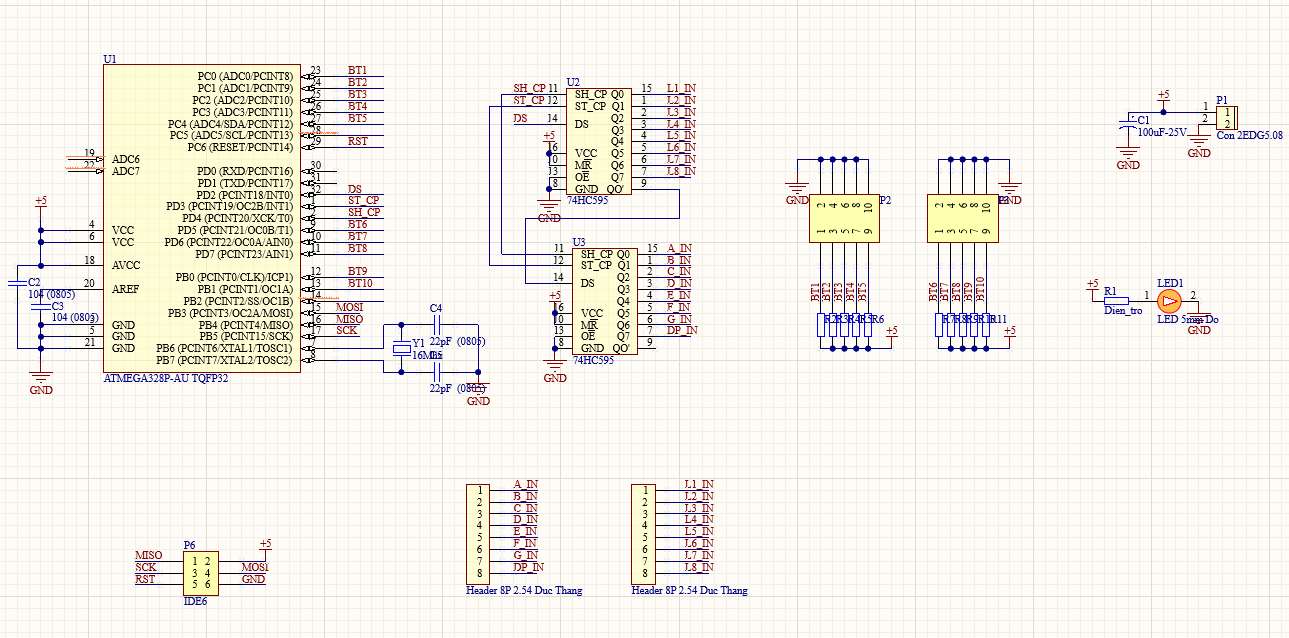
\includegraphics[width=1\textwidth]{image/sch2.png}
    \caption{Sơ đồ nguyên lý mạch điều khiển LED 7 đoạn}
    \label{fig:sodonguyenly}
\end{figure}
\begin{figure}[H]
    \centering
    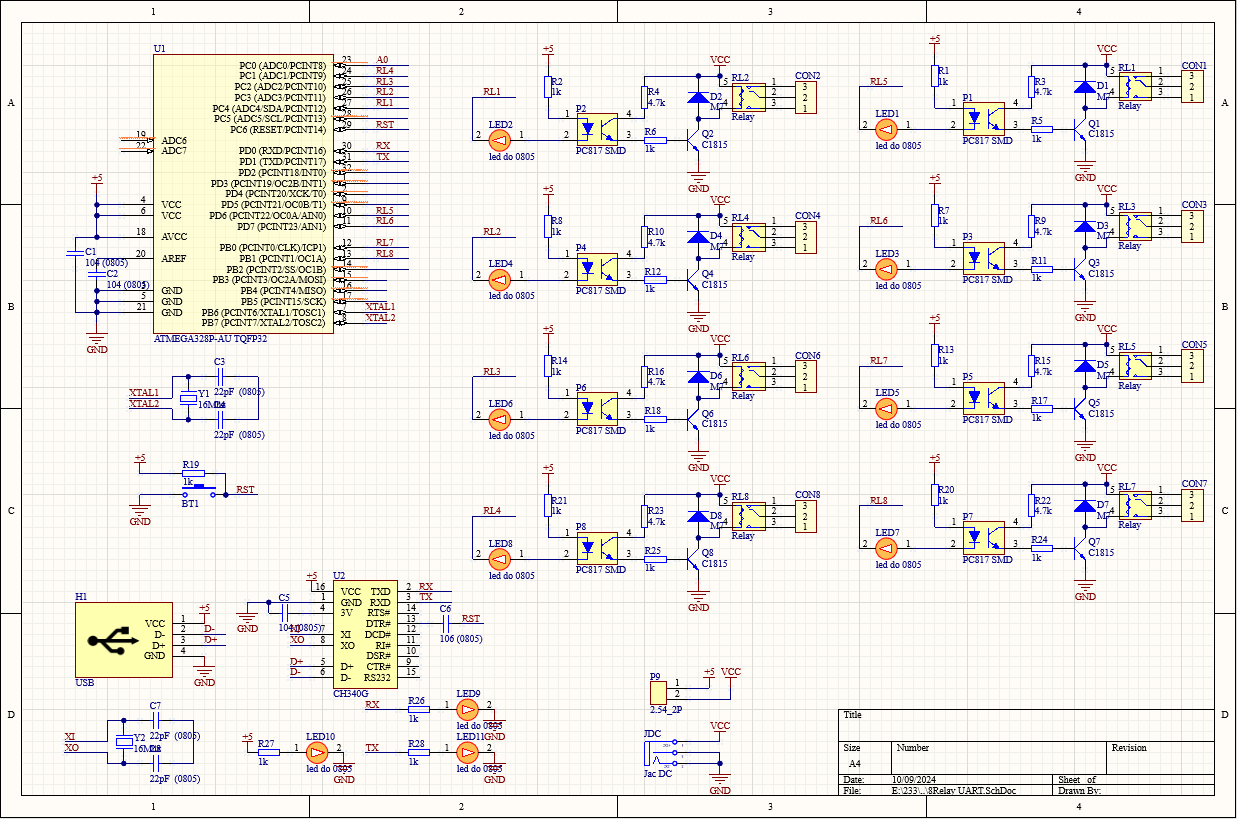
\includegraphics[width=1\textwidth]{image/sch3.png}
    \caption{Sơ đồ nguyên lý mạch điều khiển 8 relay}
    \label{fig:sodonguyenly}
\end{figure}
\begin{figure}[H]
    \centering
    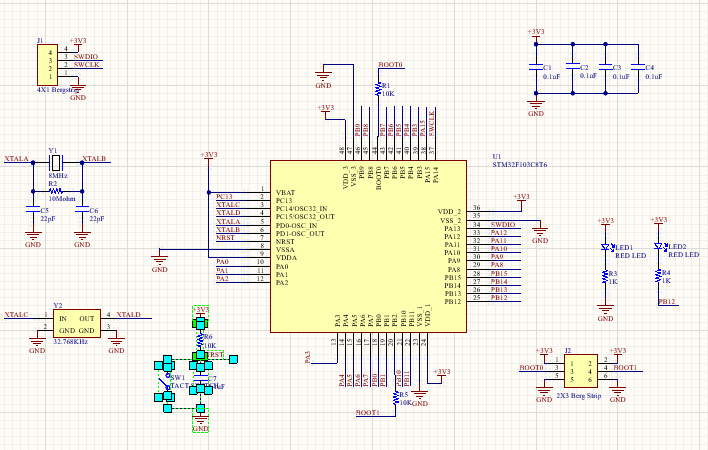
\includegraphics[width=1\textwidth]{image/sch4a.png}
    \caption{Sơ đồ nguyên lý mạch STM32F103C8T6 phần điều khiển}
    \label{fig:sodonguyenly}
\end{figure}
\begin{figure}[H]
    \centering
    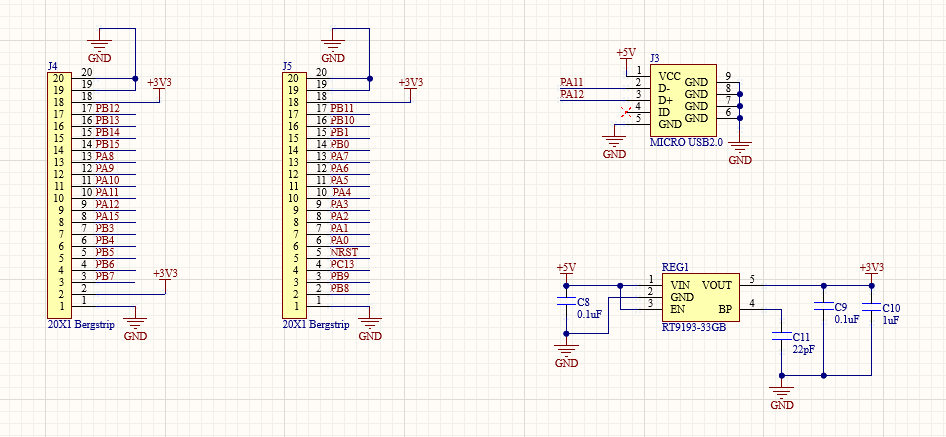
\includegraphics[width=1\textwidth]{image/4b.png}
    \caption{Sơ đồ nguyên lý mạch STM32F103C8T6 phần kết nối}
    \label{fig:sodonguyenly}
\end{figure}
\begin{figure}[H]
    \centering
    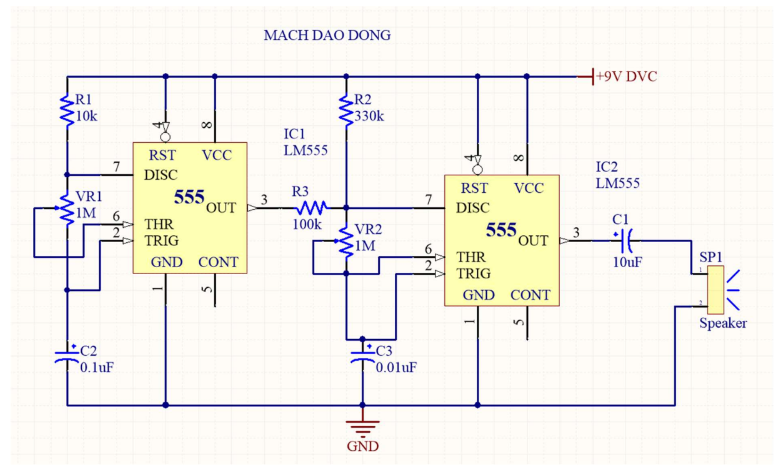
\includegraphics[width=1\textwidth]{image/sch5.png}
    \caption{Sơ đồ nguyên lý mạch dao động}
    \label{fig:sodonguyenly}
\end{figure}
\cleardoublepage
\subsection{Mạch in PCB}
\subsubsection{Sơ lược về mạch in PCB}
Sơ đồ mạch in (PCB - Printed Circuit Board) là một bản vẽ chi tiết mô tả các
thành phần và kết nối điện tử trên một bảng mạch. Để thiết kế một sơ đồ mạch in PCB,
bạn cần phải thực hiện các bước cơ bản sau: 
\begin{itemize}
    \item Xác định yêu cầu:
    \begin{itemize}
        \item Xác định các thành phần cần thiết cho mạch.
        \item Định rõ các yêu cầu về điện áp, dòng điện, và tần số.
    \end{itemize}
    \item Thiết kế sơ đồ nguyên lý (schematic):
    \begin{itemize}
        \item Vẽ sơ đồ nguyên lý để biểu diễn các thành phần điện tử và kết nối giữa chúng.
        \item Sử dụng phần mềm thiết kế mạch điện tử như Eagle, KiCad, Altium Designer,...
    \end{itemize}
    \item Chuyển sơ đồ nguyên lý thành sơ đồ mạch in (PCB layout):
    \begin{itemize}
        \item Sử dụng phần mềm thiết kế PCB để tạo ra bố trí mạch in từ sơ đồ nguyên lý.
        \item Đặt các thành phần trên bảng mạch sao cho tối ưu hóa không gian và đảm bảo hiệu quả kết nối điện.
    \end{itemize}
    \item Route các đường mạch:
    \begin{itemize}
        \item Kết nối các chân của các thành phần bằng các đường mạch trên bảng PCB.
        \item Đảm bảo các đường mạch không bị chồng chéo và tuân theo quy tắc thiết kế.
    \end{itemize}
    \item Kiểm tra và xác nhận thiết kế:
    \begin{itemize}
        \item Kiểm tra sơ đồ mạch in để đảm bảo không có lỗi.
        \item Sử dụng các công cụ kiểm tra DRC (Design Rule Check) để đảm bảo tuân thủ các quy tắc thiết kế.
    \end{itemize}
    \item Xuất file Gerber:
    \begin{itemize}
        \item Xuất các file Gerber từ phần mềm thiết kế PCB để gửi đến nhà sản xuất PCB.
        \item File Gerber là định dạng tiêu chuẩn được sử dụng trong sản xuất PCB.
    \end{itemize}
    \item Sản xuất PCB:
    \begin{itemize}
        \item Gửi các file Gerber đến nhà sản xuất PCB để họ tạo ra bảng mạch thực tế.
        \item Sau khi sản xuất, kiểm tra bảng mạch để đảm bảo chất lượng.
    \end{itemize}
\end{itemize}
\subsubsection{Ví dụ về mạch in PCB}
\begin{figure}[H]
    \centering
    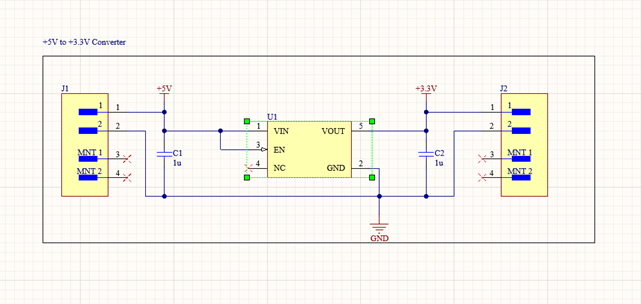
\includegraphics[width=1\textwidth]{image/sch1.png}
    \caption{Sơ đồ nguyên lý mạch chuyển đổi điện áp}
    \label{fig:sodonguyenly}
\end{figure}
\begin{figure}[H]
    \centering
    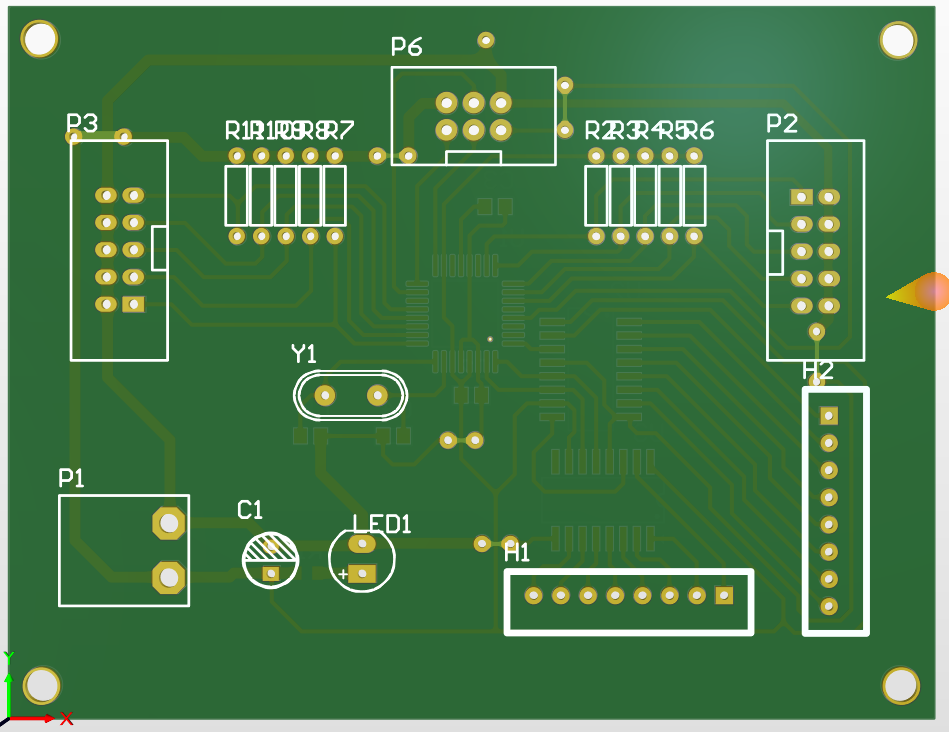
\includegraphics[width=1\textwidth]{image/pcb1.png}
    \caption{Mặt trước mạch điều khiển LED 7 đoạn}
    \label{fig:hbridge}
\end{figure}
\begin{figure}[H]
    \centering
    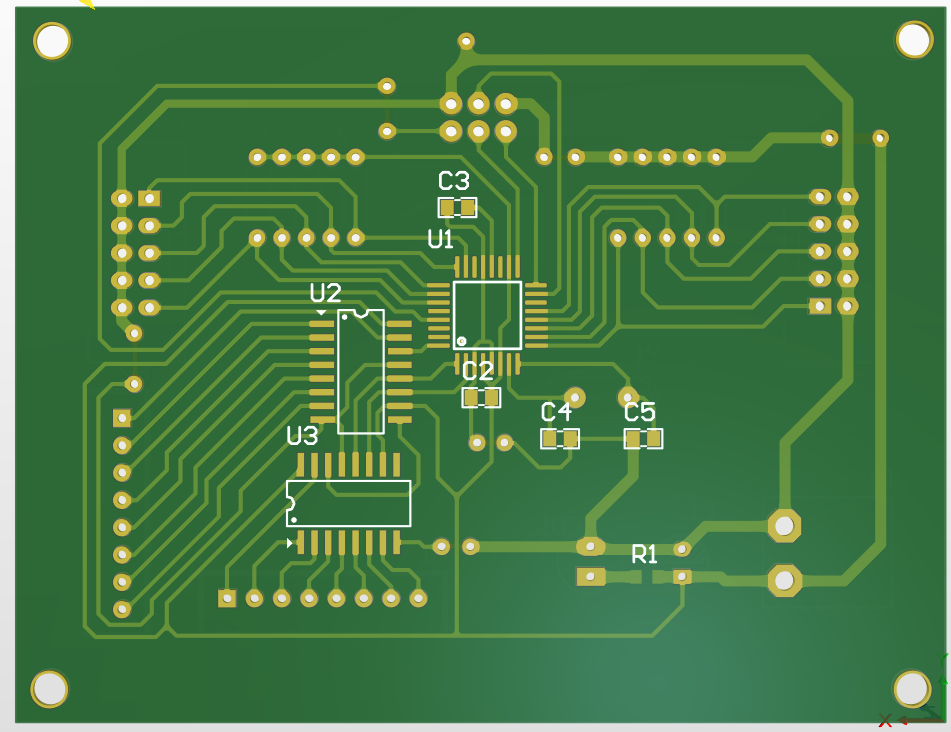
\includegraphics[width=1\textwidth]{image/pcb2.png}
    \caption{Mặt sau mạch điều khiển LED 7 đoạn}
    \label{fig:hbridge}
\end{figure}
\begin{figure}[H]
    \centering
    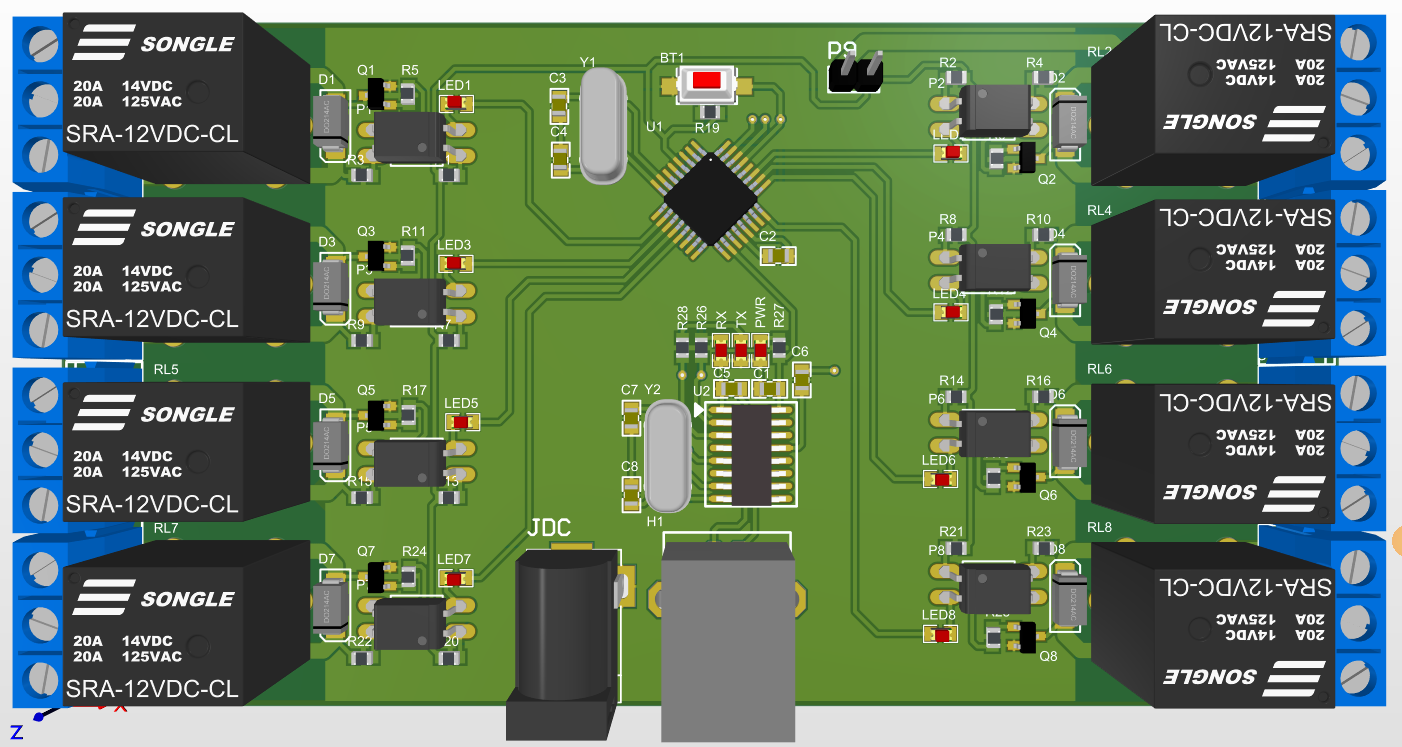
\includegraphics[width=1\textwidth]{image/pcb3.png}
    \caption{Mạch điều khiển 8 relay}
    \label{fig:hbridge}
\end{figure}
\begin{figure}[H]
    \centering
    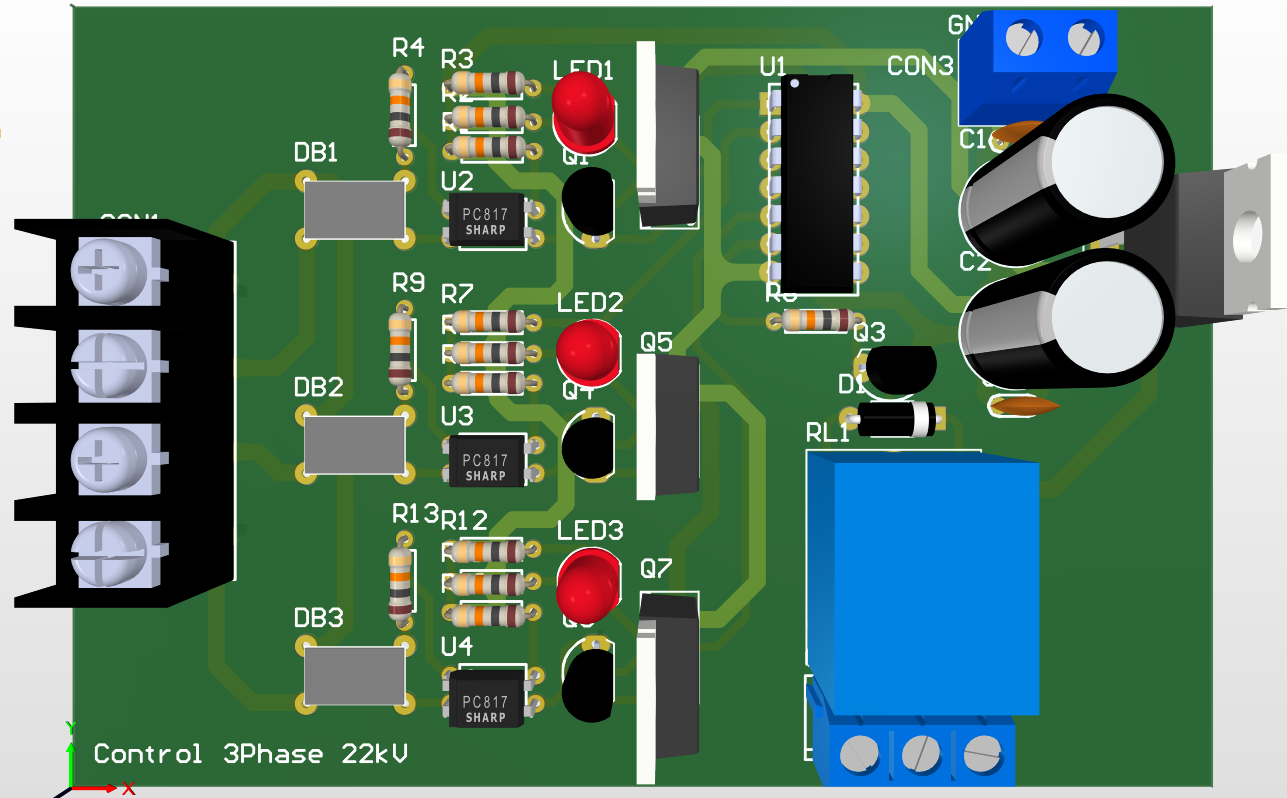
\includegraphics[width=1\textwidth]{image/pcb4.png}
    \caption{Mạch điều khiển 3 pha}
    \label{fig:hbridge}
\end{figure}
\begin{figure}[H]
    \centering
    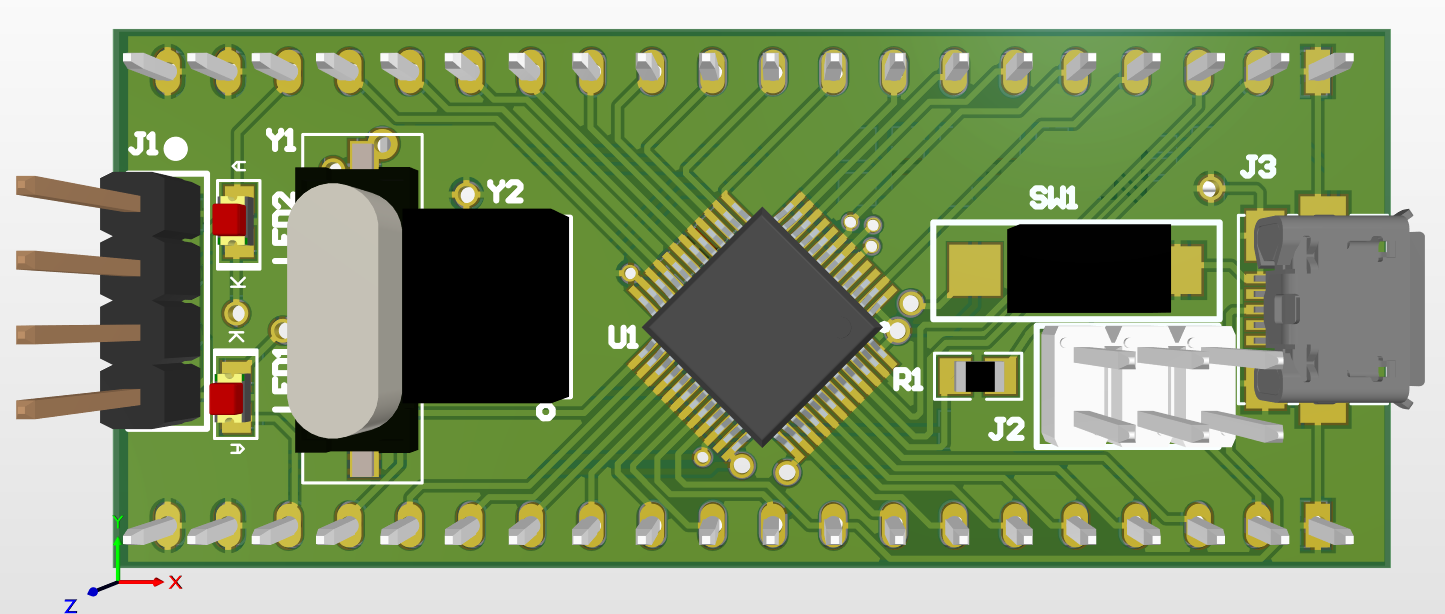
\includegraphics[width=1\textwidth]{image/pcb5.png}
    \caption{Mạch STM32F103C8T6}
    \label{fig:hbridge}
\end{figure}
\cleardoublepage
\section*{CHƯƠNG 2: MẠCH CẦU H}
\stepcounter{section}
\addcontentsline{toc}{section}{\numberline{}CHƯƠNG 2: MẠCH CẦU H}
\subsection{Cấu tạo của mạch cầu H}
Mạch cầu H là một mạch điện tử cơ bản được sử dụng rộng rãi để điều khiển hướng quay của động cơ một chiều (DC) hoặc điều khiển công suất truyền đến tải. Hình dạng mạch khi vẽ ra giống chữ H, nên được gọi là mạch cầu H.\\
Mạch cầu H, như tên gọi của nó, được thiết kế với cấu trúc cơ bản hình chữ H. Cấu tạo chính của mạch bao gồm: 
\vspace{-0.4cm}
\begin{itemize}
    \item 4 công tắc điện tử: Đây là các linh kiện chính của mạch, thường là transistor (BJT) hoặc MOSFET. Chúng đóng vai trò như những chiếc cầu nối, điều khiển dòng điện đi qua động cơ.
    \item Diode bảo vệ: Các diode được mắc song song với mỗi công tắc để bảo vệ chúng khỏi hiện tượng điện áp ngược khi các công tắc tắt.
    \item Nguồn cung cấp: Cung cấp điện áp một chiều để cấp cho mạch và động cơ.
\end{itemize}
\begin{figure}[H]
    \centering
    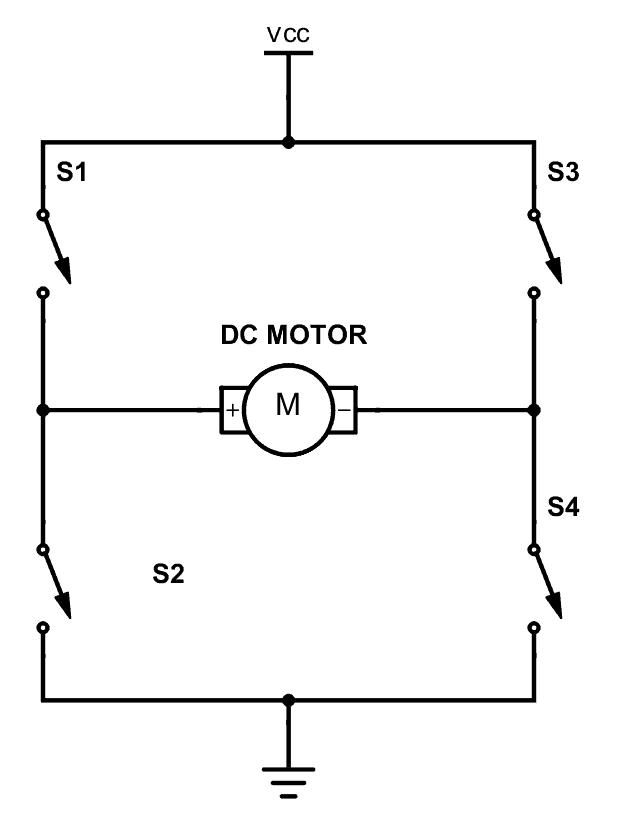
\includegraphics[width=0.5\textwidth]{image/cauhsimple.png}
    \caption{Mạch cầu H đơn giản}
    \label{fig:hbridge}
\end{figure}
\begin{figure}[H]
    \centering
    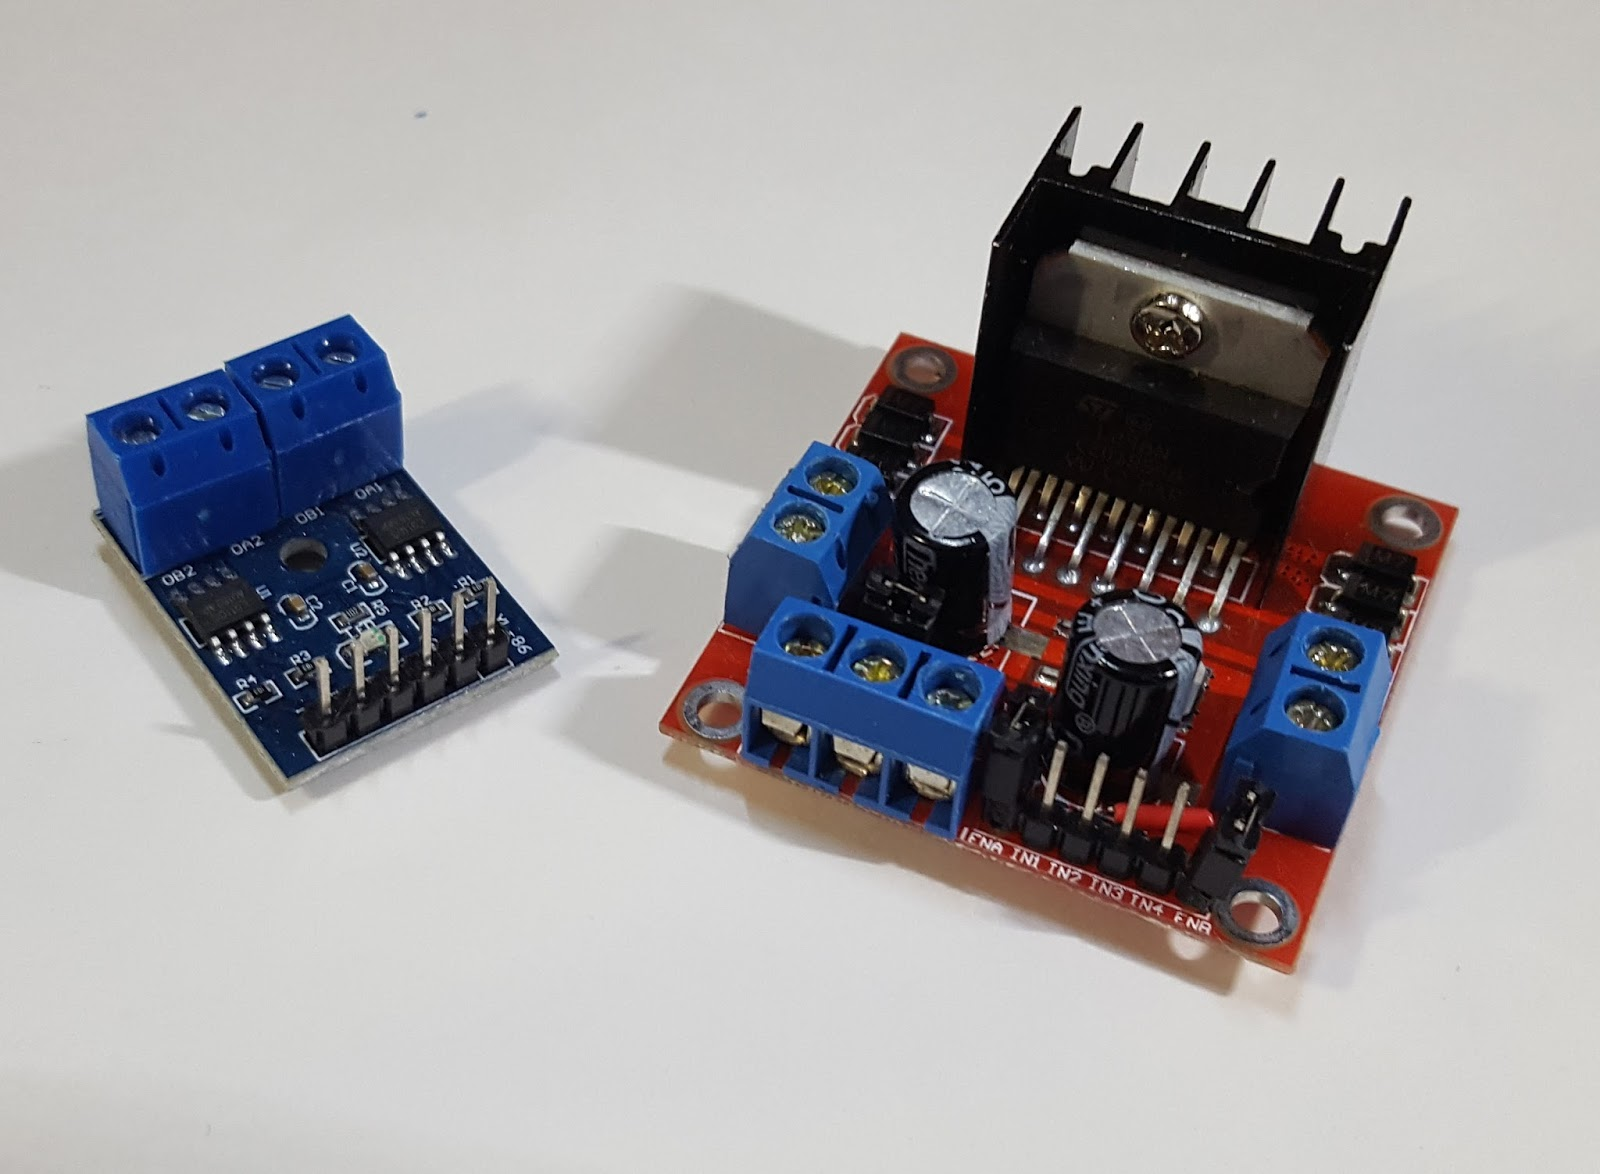
\includegraphics[width=1\textwidth]{image/cauhcurcuit.png}
    \caption{Các mô đun có tích hợp mạch cầu H}
    \label{fig:hbridge}
\end{figure}
\cleardoublepage
\subsection{Nguyên lý hoạt động của mạch cầu H}
\begin{figure}[H]
    \centering
    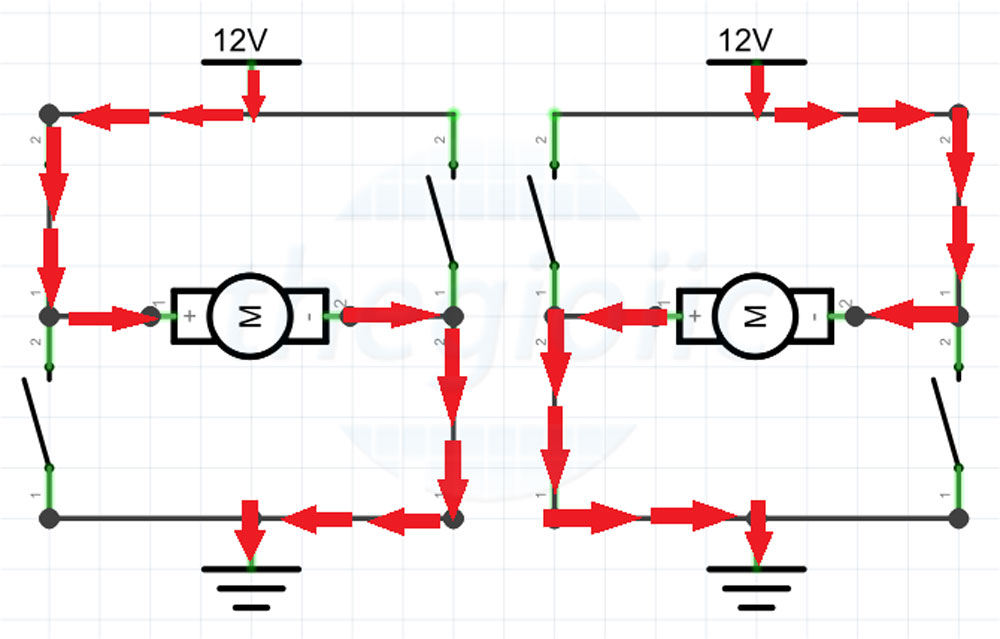
\includegraphics[width=0.8\textwidth]{image/cauhwork.png}
    \caption{Nguyên lý hoạt động của mạch cầu H}
    \label{fig:hbridge}
\end{figure}
Trong mô hình này, chúng ta sử dụng mạch cầu H để điều khiển động cơ một chiều. Động cơ DC có thể quay theo chiều thuận hoặc chiều nghịch, tùy thuộc vào cách chúng ta kết nổi cực âm và cực dương cho động cơ.

Mạch cầu H được thiết kế để điều khiển động cơ DC hoặc tải điện theo hai hướng: hướng thuận và hướng nghịch. Mạch này bao gồm bốn transistor hoặc MOSFET được kết nối với nhau theo cấu trúc dạng cầu.

Khi một cặp transistor được kích hoạt, một transistor ở phía trên và một transistor ở phía dưới, dòng điện sẽ chảy qua động cơ theo hướng tương ứng. Khi cặp transistor khác được kích hoạt, hướng dòng điện sẽ đảo ngược, từ đó điều khiển tải đi theo hướng khác

Việc điều khiển được thực hiện thông qua các cổng điều khiển được kết nối đến bồn transistor hoặc MOSFET, khi điện áp được đưa vào các cổng này, các transistor sẽ được kích hoạt hoặc ngưng hoạt động tùy thuộc vào tín hiệu đầu vào tại cổng.
\cleardoublepage
\subsection{Ứng dụng mạch cầu H trong thực tế}
Bên cạnh việc điều khiển động cơ DC, mạch cầu H còn được sử dụng rộng rãi trong các ứng dụng khác như:
\begin{itemize}
    \item Điều khiển động cơ servo: Mạch cầu H cũng được sử dụng để điều khiển động cơ servo trong các ứng dụng yêu cầu độ chính xác cao như robotica, máy bay điều khiển từ xa và các thiết bị tự động hóa khác.
    \item Hệ thống quản lý năng lượng: Mạch cầu H được tích hợp vào hệ thống quản lý năng lượng để điều khiển việc cung cấp năng lượng cho các thiết bị điện tử như ổ đĩa động cơ, hệ thống điều hòa không khí và thiết bị gia dụng.
    \item Hệ thống truyền dẫn điện không dây: Trong các ứng dụng truyền dẫn điện không dây như sạc không dây cho điện thoại di động, mạch cầu H có thể được sử dụng để điều khiển nguồn điện được truyền từ trạm sạc đến thiết bị di động.
    \item Hệ thống giao thông thông minh: Trong các hệ thống giao thông thông minh, mạch cầu H có thể được sử dụng để điều khiển các thiết bị như cổng xoay, cửa tự động và đèn tín hiệu giao thông để tạo ra một mạng lưới giao thông hiệu quả và an toàn.
\end{itemize}
\begin{figure}[H]
    \centering
    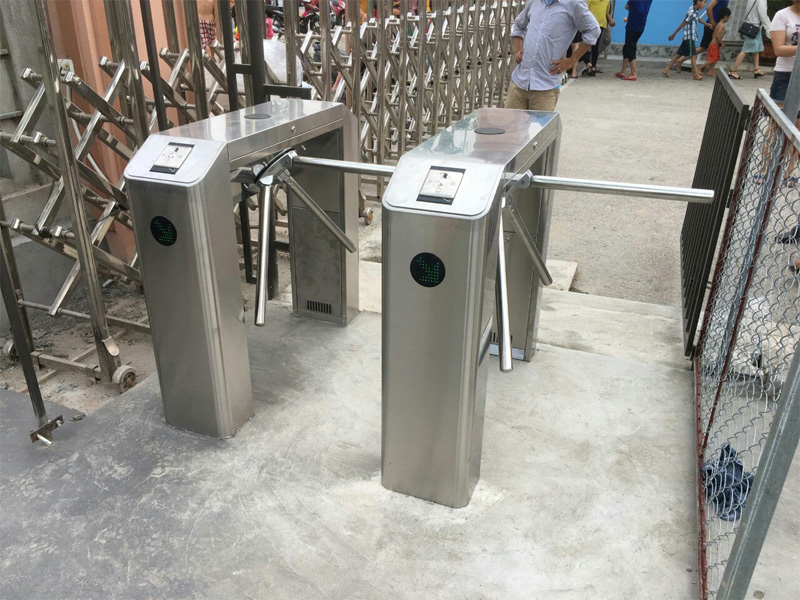
\includegraphics[width=1\textwidth]{image/cong3que.png}
    \caption{Hệ thống cổng xoay 3 càng có sử dụng mạch cầu H}
    \label{fig:hbridge}
\end{figure}
\cleardoublepage

\cleardoublepage
\end{document}